\chapter{TINJAUAN PUSTAKA}
\vspace{1ex}

\section*{}
Demi mendukung penelitian ini, dibutuhkan beberapa teori penunjang sebagai bahan acuan dan referensi. Dengan demikian penelitian ini menjadi lebih terarah. 
\vspace{1ex}

\section{Simulator Berkendara / \textit{Driving Simulator}}
\vspace{1ex}

\textit{Driving Simulator} atau \textit{Simulator Berkendara}  adalah penggambaran suatu sistem atau proses berkendara dengan peragaan menyerupai proses atau kegiatan berkendara sesungguhnya. \textit{Driving simulator} dapat digunakan untuk kegiatan hiburan, serta juga dapat digunakan untuk kegiatan riset yang mana dapat digunakan untuk memonitor perilaku pengemudi, kinerja, serta perhatian dari pengemudi yang sedang diuji pada simulator tersebut. \cite{cit:11}
\vspace{1ex}

\section{\textit{Perception Time} (PR)}
\vspace{1ex}

\textit{Perception Time} (PR) merupakan istilah yang di ciptakan untuk mengukur tingkat kewaspadaan pengemudi. Perhitungan PR, adalah waktu yang dibutuhkan dari terlihatnya halangan tidak terduga hingga waktu yang dibutuhkan oleh pengemudi untuk menekan pedal gas untuk berhenti. PR adalah faktor penting yang telah digunakan oleh para arsitek untuk mendesain serta membangun jalan raya. \cite{cit:8}
\vspace{1ex}

\section{Tingkat Kantuk Subjektif dan Objektif \textit{(Subjective and Objective Sleepiness)}}
\vspace{1ex}

\textit{Subjective sleepiness} atau tingkat kantuk subjektif perlu dibedakan dengan \textit{Objective Sleepiness} atau tingkat kantuk objektif, hal ini dikarenakan untuk mendeteksi pengemudi yang sedang kelelahan diperlukan fitur - fitur objektif oleh suatu sistem sehingga dapat digunakan sebagai dataset untuk sistem deteksi tersebut. Paper ini mengajukan bagaimana cara untuk mendapatkan fitur - fitur \textit{objective sleepiness} tersebut\cite{cit:5}
\vspace{1ex}

\section{\textit{Bézier curve}}
\vspace{1ex}

\begin{figure} [!htb]
	\captionsetup{justification=centering}
	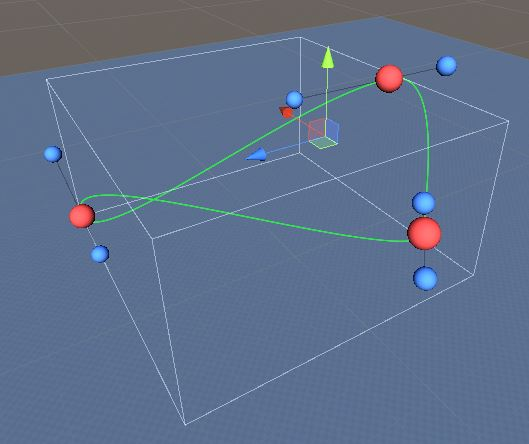
\includegraphics[scale=0.4]{img/contoh-kurva-bezier.JPG}
	\caption{Contoh kurva bezier pada bidang 3 dimensi}
	\label{fig:2.1}
\end{figure}

\textit{Bézier curve} atau kurva bezier adalah kurva parametrik yang banyak digunakan pada bidang grafika komputer serta bidang - bidang lain yang berhubungan. Sifat dari kurva bezier yang parametrik dapat digunakan untuk memodelkan kurva pada 2 atau bahkan 3 dimensi grafika komputer. Selain itu sifat parametrik ini juga membawa sifat lain yang mana menyebabkan kurva bezier memiliki sifat dapat diskalakan sesuai dengan kebutuhan. Kurva bezier memiliki 2 komponen utama, yaitu \textit{control points} atau titik kontrol, serta \textit{anchor points} atau titik jangkar Dengan menentukan lokasi serta orientasi (apabila pada 3 dimensi) dari titik - titik kontrol dan titik jangkar yang digunakan pada kurva bezier, sehingga dapat dimodelkan seluruh jenis kurva dengan mudah, serta pada penerapan di grafika komputer, cukup mudah dalam melakukan operasi transformasi pada titik - titik kontrol untuk mendapatkan jenis kurva yang diinginkan.\cite{cit:9}

\section{\textit{6 Degree of Freedom}}
\vspace{1ex}

\begin{figure}  [!htb]
	        \captionsetup{justification=centering}
	        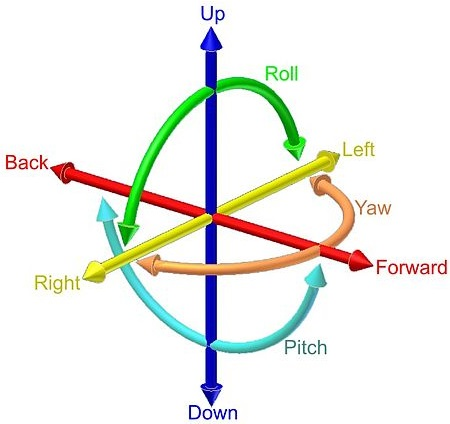
\includegraphics[scale=0.4]{img/6dof.jpg}
	        \caption{\textit{6 Degrees of Freedom - Pitch, Roll,} dan \textit{Yaw}\cite{cit:15}}
	        \label{fig: 3_18}
\end{figure}

\textit{6 Degree of Freedom / DoF}, adalah istilah atau penjelasan dari pergerakan suatu objek pada dimensi spasial ketiga. \textit{DoF} memiliki 3 macam istilah yang perlu di ketahui, Yang pertama \textit{Pitch} ialah merepresentasikan sudut putaran terhadap sumbu \textit{x}, yang kedua \textit{Yaw}, yang merepresentasikan sudut putaran terhadap sumbu \textit{y}, yang ketiga \textit{Roll}, yang merepresentasikan sudut putaran terhadap sumbu \textit{z}.

\section{Kecepatan / \textit{Velocity}}
\vspace{1ex}

\begin{figure}  [!htb]
	        \captionsetup{justification=centering}
	        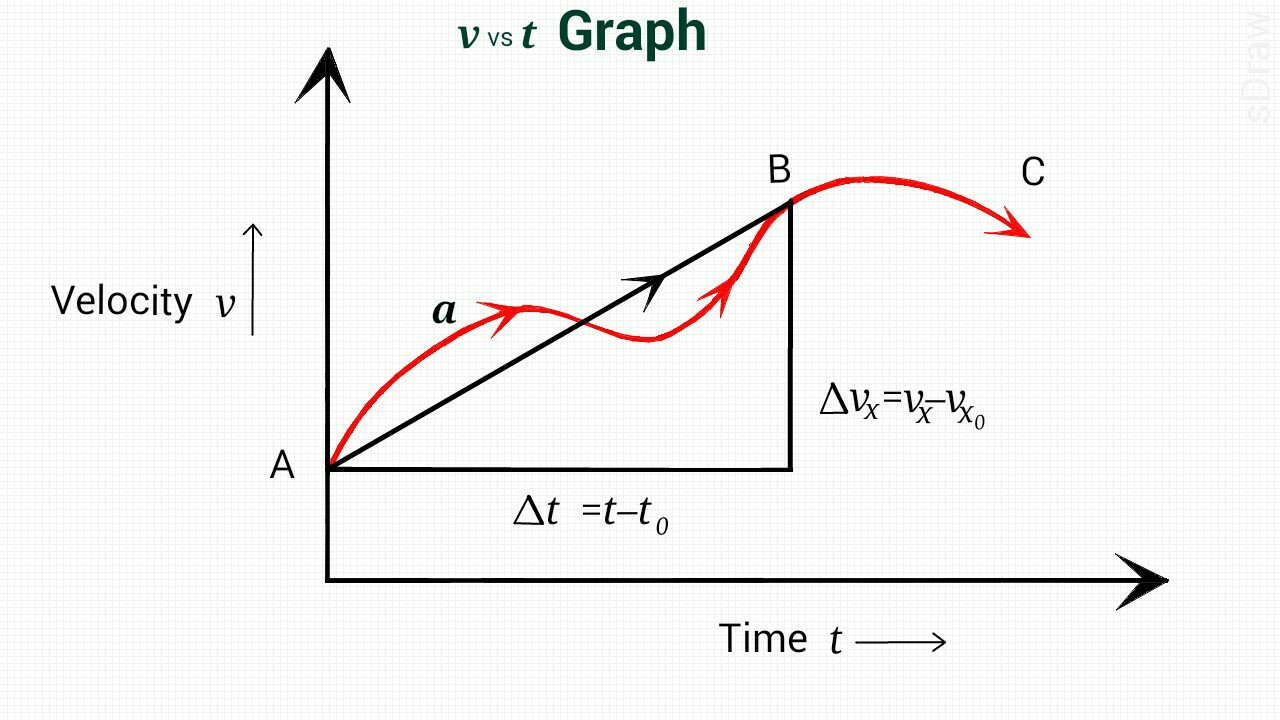
\includegraphics[scale=0.2]{img/velocity.jpg}
        	%\caption{Diagram alur kerja}
        	\caption{Kecepatan}
        	\label{fig: 3_27}
\end{figure}

Kecepatan / \textit{velocity} pada bidang grafika komputer, terdapat 2 jenis yaitu: kecepatan vektor serta besaran kecepatan, kecepatan vektor ialah seberapa unit jauh objek berpindah dalam suatu hitungan waktu terhadap masing - masing sumbu x, y, serta z.

\section{\textit{Colission}}
\vspace{1ex}

Konsep \textit{Collission} pada \textit{Unity Game Engine}, ialah terdapat 2 macam \textit{collider}. \textit{Collider} itu sendiri ialah entitas yang dapat berinteraksi dengan \textit{collider lain}. 2 Macam \textit{collider} adalah \textit{trigger collider} serta \textit{physics collider}. \textit{Physics collider} ialah entitas \textit{collider} yang mensimulasikan hukum fisika dengan akurat, seperti contohnya interaksi roda dengan jalan/tanah, mobil dengan mobil lain, dsb. Sedangkan \textit{Trigger Collider} tidak mensimulasikan hal tersebut, fungsi dari \textit{trigger collider} ialah \textit{unity} dapat mengetahui bahwa suatu entitas \textit{collider} lain telah berinteraksi dengan \textit{trigger collider} tersebut, sehingga dapat melakukan perintah terprogram menggunakan \textit{event system}